\documentclass[12pt,a4paper]{report}
\usepackage[utf8]{inputenc}
\usepackage[spanish]{babel}
\usepackage{amsmath}
\usepackage{amsfonts}
\usepackage{amssymb}
\usepackage{makeidx}
\usepackage{graphicx}
\usepackage[hidelinks]{hyperref}
\usepackage[left=2cm,right=2cm,top=2cm,bottom=2cm]{geometry}
\usepackage{hyperref}



\begin{document}

\author{Fonseca Camarena Jonathan}

\title{\begin{center}

\includegraphics[scale=1.5]{Escudo.png} 
\end{center}Explicar el operador Jacobiano}

\date{
Universidad Politécnica de la Zona Metropolitana de Guadalajara\\
Profesor: Carlos Enrique Morán Garabito\\
30 de septiembre del 2019}

\maketitle
\tableofcontents
\section{Introducción}
En cálculo vectorial, se llama jacobiano o determinante jacobiano al determinante de la matriz jacobiana. Tanto la matriz jacobiana como el determinante jacobiano reciben su nombre en honor al matemático Carl Gustav Jacobi.
\noindent\\
En geometría algebraica, el jacobiano de una curva hace referencia a la variedad jacobiana, un grupo y variedad algebraica asociada a la curva, donde la curva puede ser embebida.

\section{Matriz Jacobiano}
La matriz jacobiana es una matriz formada por las derivadas parciales de primer orden de una función. Una de las aplicaciones más interesantes de esta matriz es la posibilidad de aproximar linealmente a la función en un punto. En este sentido, el jacobiano representa la derivada de una función multivariable. 
\noindent\\
Propiamente deberíamos hablar más que de matriz jacobiana de diferencial jacobiana o aplicación lineal jacobiana ya que la forma de la matriz dependerá de la base o coordenadas elegidas. Es decir, dadas dos bases diferentes la aplicación lineal jacobiana tendrá componentes diferentes aun tratándose del mismo objeto matemático. 
\section{Operador Jacobiano}
Para la obtención del operador Jacobiano, se deben tener las velocidades lineal y angular de cada uno de los planos del sistema de robot de tres grados de libertad, con el método de la velocidad de propagación.

•	Velocidades del primer plano\\
La velocidad angular del plano cero es nula, ya que no tiene niguna rotación por ser el plano de referencia para los demás planos. Remplazando
\vspace{25mm} %5mm vertical space
 \hspace{1cm}\hspace{1cm} 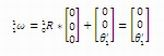
\includegraphics{ecuacion1.jpg}
 

•	Velocidad lineal\\
En el primer plano no existe de movimiento de translación por consiguiente la velocidad lineal es cero.

 \hspace{6cm} 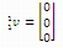
\includegraphics{ecuacion2.jpg}

  
Velocidades del segundo plano:\\
•	Velocidad angular\\

   \hspace{2cm}  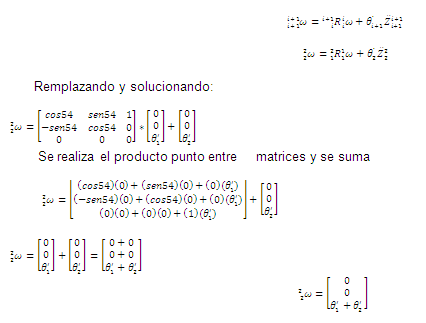
\includegraphics{ecuacion3.png}
   
   
Velocidad lineal:\\

   \hspace{5cm} 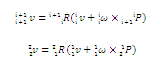
\includegraphics{ecuacion4.png}\\
   
   \vspace{50mm} %5mm vertical space
Solución del producto cruz
   
     
   \hspace{4cm} 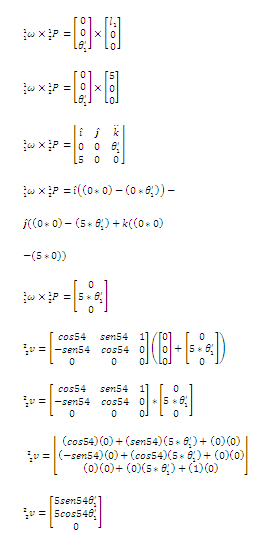
\includegraphics{ecuacion5.png}\\
   
Velocidades del tercer plano
•	Velocidad angular
AL tener el mismo ángulo de rotación el plano tres con el dos la velocidad angular es igual.\\

  
   \hspace{4cm} 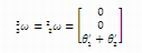
\includegraphics{ecuacion6.jpg}\\
   
   
Velocidad Lineal

   
  \hspace{4cm} 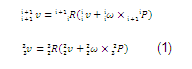
\includegraphics{ecuacion7.png}\\
  
  Solución del Producto de Cruz
  
  
  \hspace{4cm} 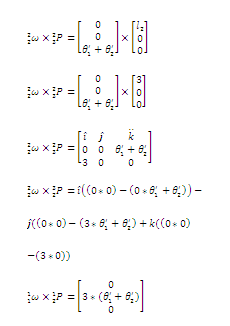
\includegraphics{ecuacion8.png}\\
  
  Remplazando en la ecuación (1)
  
  
  \hspace{4cm} 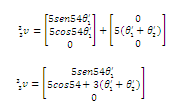
\includegraphics{ecuacion9.png}\\
  
  Por tanto el Jacobiano expresado en el plano tres es:
  
   \hspace{4cm} 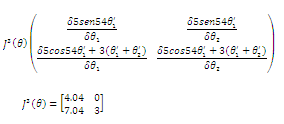
\includegraphics{ecuacion10.png}\\
  
  La velocidad del plano tres expresada en el plano de referencia cero:
  
  \hspace{4cm} 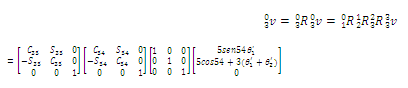
\includegraphics{ecuacion11.png}\\
  
  Se realiza el producto entre las matrices
  
  \hspace{4cm} 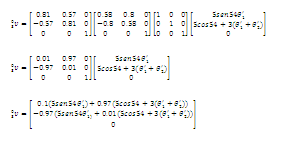
\includegraphics{ecuacion12.png}\\
  
  El Jacobiano expresado en 3 es:
  

  
  \hspace{4cm} 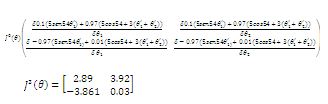
\includegraphics{ecuacion13.png}\\
  
  El vector es la relación de las velocidades articulares con las velocidades cartesianas del extremo.
  
  \section{Conclusión}
  Esta investigació permite explicar con un cálculo concreto la velocidad de las articulaciones de un robot   manipulador, sin importar cuantas tenga, y permite la relación de la velocidad angular y lineal.
  Mas complicado que las tareas pasadas, en las siguientes practicas pondremos a prueba los conocimiientos antes mencionados.
  
\cite{ollero}
\bibliographystyle{plain}
\bibliography{ollero}  

\end{document}
